% ---- pg-474 （书页 462） ----

\phantomsection\label{eq:11-28}
\begin{equation}
k=\frac{1}{2}\ln\left(\frac{|\boldsymbol{\Sigma}_1|}{|\boldsymbol{\Sigma}_2|}\right)+\frac{1}{2}(\boldsymbol{\mu}_1'\boldsymbol{\Sigma}_1^{-1}\boldsymbol{\mu}_1-\boldsymbol{\mu}_2'\boldsymbol{\Sigma}_2^{-1}\boldsymbol{\mu}_2)
\tag{11-28}
\end{equation}
这些分类域由 $\mathbf{x}$ 的二次函数定义. 当 $\boldsymbol{\Sigma}_1=\boldsymbol{\Sigma}_2$ 时, 二次项 $-\frac{1}{2}\mathbf{x}'(\boldsymbol{\Sigma}_1^{-1}-\boldsymbol{\Sigma}_2^{-1})\mathbf{x}$ 消失, 于是由\hyperref[eq:11-27]{式(11-27)}所定义的区域退化为由\hyperref[eq:11-14]{式(11-14)}所定义的区域.

一般多元正态总体的分类法则直接由\hyperref[eq:11-27]{式(11-27)}得到.

\noindent\textbf{结论 11.4}\quad 设总体 $\pi_1$ 和 $\pi_2$ 由均值向量和协方差矩阵分别为 $\boldsymbol{\mu}_1$, $\boldsymbol{\Sigma}_1$ 和 $\boldsymbol{\mu}_2$, $\boldsymbol{\Sigma}_2$ 的正态密度所刻画, 则能使期望错分代价(ECM)达到最小的分配法则为:

当
\[
-\frac{1}{2}\mathbf{x}_0'(\boldsymbol{\Sigma}_1^{-1}-\boldsymbol{\Sigma}_2^{-1})\mathbf{x}_0+(\boldsymbol{\mu}_1'\boldsymbol{\Sigma}_1^{-1}-\boldsymbol{\mu}_2'\boldsymbol{\Sigma}_2^{-1})\mathbf{x}_0-k\geqslant\ln\left[\left(\frac{c(1\mid2)}{c(2\mid1)}\right)\left(\frac{p_2}{p_1}\right)\right]
\]
时将 $\mathbf{x}_0$ 分配给 $\pi_1$, 否则将 $\mathbf{x}_0$ 分配给 $\pi_2$.

这里 $k$ 由\hyperref[eq:11-28]{式(11-28)}所给出.

在实践中, 结论 11.4 中的分类法则是通过用样本量 $\bar{x}_1$, $\bar{x}_2$, $\mathbf{S}_1$ 和 $\mathbf{S}_2$[见\hyperref[eq:11-16]{式(11-16)}]分别代替总体量 $\boldsymbol{\mu}_1$, $\boldsymbol{\mu}_2$, $\boldsymbol{\Sigma}_1$ 和 $\boldsymbol{\Sigma}_2$ 来实施的.\footnote{为保证 $\mathbf{S}_1^{-1}$ 和 $\mathbf{S}_2^{-1}$ 存在, 不等式 $n_1>p$ 和 $n_2>p$ 都必须成立, 因为这样才能用 $\mathbf{S}_1^{-1}$ 和 $\mathbf{S}_2^{-1}$ 分别取代 $\boldsymbol{\Sigma}_1^{-1}$ 和 $\boldsymbol{\Sigma}_2^{-1}$, 从而得出样本分类法则(11-29).}

\begin{mvframe}[二次分类法则(有不同协方差阵的正态总体)]
若
\phantomsection\label{eq:11-29}
\begin{equation}
-\frac{1}{2}\mathbf{x}_0'(\mathbf{S}_1^{-1}-\mathbf{S}_2^{-1})\mathbf{x}_0+(\bar{\mathbf{x}}_1'\mathbf{S}_1^{-1}-\bar{\mathbf{x}}_2'\mathbf{S}_2^{-1})\mathbf{x}_0-k\geqslant\ln\left[\left(\frac{c(1\mid2)}{c(2\mid1)}\right)\left(\frac{p_2}{p_1}\right)\right]
\tag{11-29}
\end{equation}
则将 $\mathbf{x}_0$ 分配到 $\pi_1$, 否则将 $\mathbf{x}_0$ 分配到 $\pi_2$.
\end{mvframe}

在维数大于 2 的场合, 用二次函数进行分类相当困难, 而且会导致某些奇怪的结果. 尤其当数据(本质上)不服从正态分布时, 情况更是如此.

\hyperref[fig:11.6]{图 11.6}(a)显示了建立在具有两个不同方差的分布这一理想化情况基础上的相同代价及相同先验概率法则. 在这个场合, 这个二次分类法则导致区域 $R_1$ 由两个不相联结的集合组成.

在许多应用中, $\pi_1$ 分布的左尾部分比正态分布所描述的左尾部分要低. 于是正如同\hyperref[fig:11.6]{图 11.6}(b)所示的那样, 由二次法则产生的 $R_1$ 的左尾部分不能清晰地区分两个总体分布, 因此会导致较大的失误率. 二次法则的一个严重的弱点是对偏离正态性很敏感.

\begin{mvfigure}
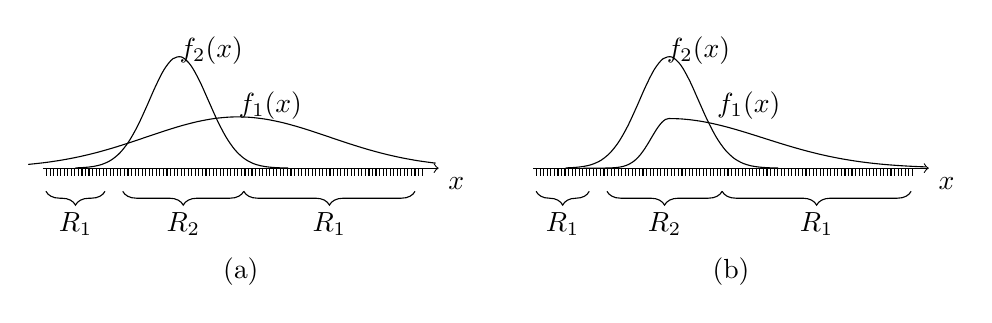
\begin{tikzpicture}[xscale=0.75,yscale=1.05]
% ================= (a) =================
\begin{scope}
  \draw[->] (0,0) -- (6.7,0) node[below right]{$x$};
  \foreach \x in {0.06,0.12,...,6.42}{\draw (\x,0) -- (\x,-0.09);}
  \draw[domain=0.55:4.15,smooth,variable=\x] plot (\x,{1.35*exp(-((\x-2.3)*(\x-2.3))/(2*0.50*0.50))});
  \draw[domain=-0.25:6.65,smooth,variable=\x] plot (\x,{0.62*exp(-((\x-3.3)*(\x-3.3))/(2*1.55*1.55))});
  \node at (2.85,1.42) {$f_2(x)$};
  \node at (3.85,0.76) {$f_1(x)$};
  \draw[decorate,decoration={brace,amplitude=5pt,mirror}] (0.05,-0.28) -- (1.05,-0.28) node[midway,below=4pt]{$R_1$};
  \draw[decorate,decoration={brace,amplitude=5pt,mirror}] (1.35,-0.28) -- (3.40,-0.28) node[midway,below=4pt]{$R_2$};
  \draw[decorate,decoration={brace,amplitude=5pt,mirror}] (3.40,-0.28) -- (6.30,-0.28) node[midway,below=4pt]{$R_1$};
  \node at (3.35,-1.25) {(a)};
\end{scope}
% ================= (b) =================
\begin{scope}[xshift=8.3cm]
  \draw[->] (0,0) -- (6.7,0) node[below right]{$x$};
  \foreach \x in {0.06,0.12,...,6.42}{\draw (\x,0) -- (\x,-0.09);}
  \draw[domain=0.55:4.15,smooth,variable=\x] plot (\x,{1.35*exp(-((\x-2.3)*(\x-2.3))/(2*0.50*0.50))});
  \draw[domain=0.85:2.3,smooth,variable=\x] plot (\x,{0.60*exp(-((\x-2.3)*(\x-2.3))/(2*0.30*0.30))});
  \draw[domain=2.3:6.65,smooth,variable=\x] plot (\x,{0.60*exp(-((\x-2.3)*(\x-2.3))/(2*1.60*1.60))});
  \node at (2.80,1.42) {$f_2(x)$};
  \node at (3.65,0.76) {$f_1(x)$};
  \draw[decorate,decoration={brace,amplitude=5pt,mirror}] (0.05,-0.28) -- (0.95,-0.28) node[midway,below=4pt]{$R_1$};
  \draw[decorate,decoration={brace,amplitude=5pt,mirror}] (1.25,-0.28) -- (3.20,-0.28) node[midway,below=4pt]{$R_2$};
  \draw[decorate,decoration={brace,amplitude=5pt,mirror}] (3.20,-0.28) -- (6.40,-0.28) node[midway,below=4pt]{$R_1$};
  \node at (3.35,-1.25) {(b)};
\end{scope}
\end{tikzpicture}
\phantomsection\label{fig:11.6}\mvcap{图 11.6\quad 二次法则: (a) 两个方差不同的正态分布; (b) 两个分布, 其中一个为非正态分布——法则不适当}
\end{mvfigure}
